\subsection{PIR-sensor}

PIR-sensoren (HC-SR501) er et færdigbygget komponent. Den har tre tilslutningsben et til 5 Vdc, et til ground og et output ben der giver signal ved bevægelse. Der er mulighed for at indstille følsomheden og forsinkelse via to potmetre. Jumperen indstiller hvordan PIR-sensoren skal trigge, ved ''L'' trigger den en enkelt gang og ved ''H'' trigger den flere gange. På figur \ref{lab:pir_overview} ses hvor de forskelle ting er placeret på bagsiden af PIR-sensoren. Driver beskrivelse og nærmere indblik i PIR-sensoren kan findes i projektdokumentationen se afsnit 5.3, PIR-sensor

\begin{figure}[H] \centering
{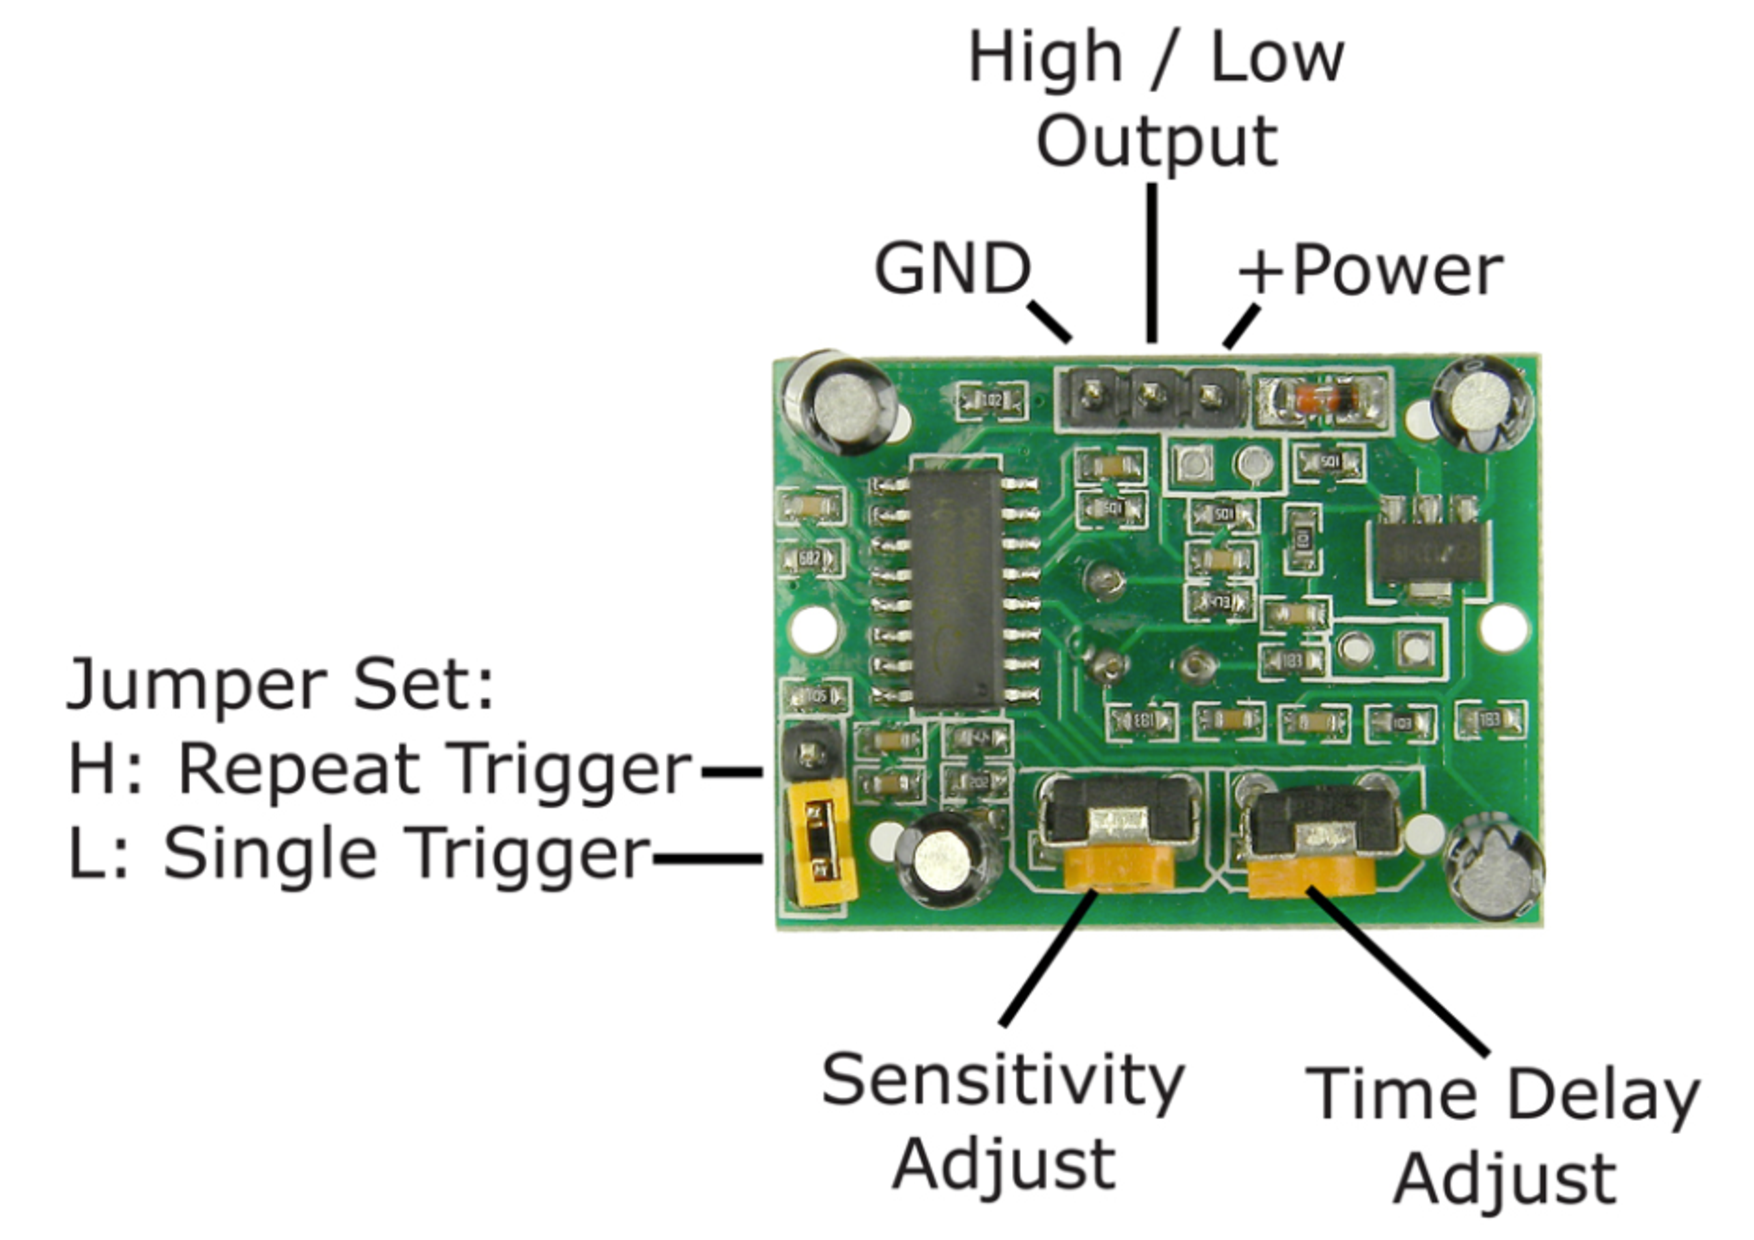
\includegraphics[width=0.5\textwidth]{Billeder/pir_overview}}
\caption{Billede af selve printet og dets indstillingsmuligheder}
\label{lab:pir_overview}
\raggedright
\end{figure}



